\section{High level Architecture}
\label{fig:architecture_diagram}
\begin{figure}[t]
\centering
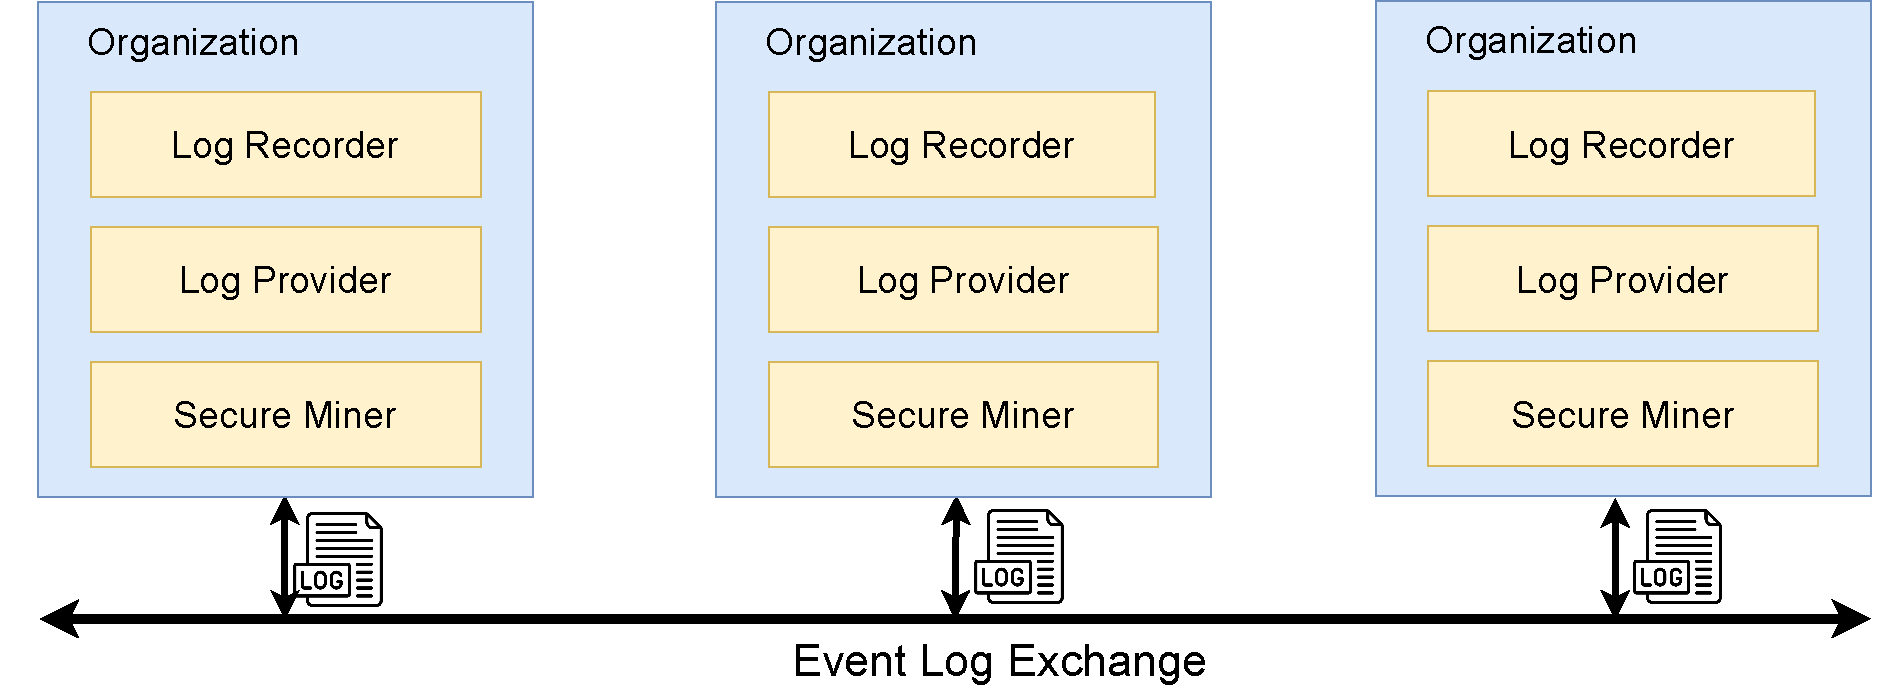
\includegraphics[width=11cm]{content/figures/architecture_diagram.pdf}
\caption{High-level architectural overview of the framework.}
\label{fig:implementation}
\end{figure}
In the following section we present the high level architecture underlying our solution. Therefore, we take into account each component individually. Subsequently, we provide an overview on the main interactions taking place between the introduced components.
\subsection{Main components}
Our architecture involve networks of nodes controlled by different \texttt{Organization}s exchanging their event logs. \texttt{Organization}s in the same network collaborate to reach a common objective composing business processes whose event logs are defraged over multiple places. The hospital and the specialized clinic, mentioned in the running example, provide an example of partner organizations. An \texttt{Organization} assumes simultaneously two different roles. We refer to an \texttt{Organization} as a \textit{miner} when it applies process mining algorithms using local event logs in combination with ones generated by partner \texttt{Organization}s. When an \texttt{Organization} deliver event logs to be mined, we call it \textit{provider}. Each \texttt{Organization} is associated with an asymetric key couple thanks to which it authenticates and makes authenticable messages from/to other \texttt{Organizations}.

In \cref{fig:architecture_diagram}, we propose an high level schematization of our solution. Each \texttt{Organization} embeds three main components: the \texttt{ERP Interface}, the \texttt{Log Provider} and the \texttt{Trusted Miner}. In the next paragraph, we address the newly mentioned components.
\subsubsection{ERP Interface}
The \texttt{ERP Interface} collects the logic to interact with the Enterprise Resource Planning (ERP) system  of the \texttt{Organization}. ERP systems helps \texttt{Organizations} to
handle business processes including accounting and resource management. The mantainance of event logs is one of the many tasks performed by these systems. In our architecture, we generalize the interaction with these systems through the \texttt{ERP Interface}. The \texttt{ERP Interface} provides the local \texttt{Log Provider} and \texttt{Trusted Miner} access to event logs generated inside the \texttt{Organization}.
\subsubsection{Log Provider}
The \texttt{Log Provider} component delivers on-demand data to \texttt{Trusted Miner}s belonging to partner \texttt{Organization}s. It handles event log request through access control methodologies, thanks to which the identity of the miner is determined and the access to the resource is decided.

\texttt{Log Provider}s authenticate event log requests using asymetric encryption methodologies. Through the latter, \texttt{Log Provider}s verifiy parameters embedded in the data request. The goal of the authentication procedure is to extract the public key representing the identity of the sender \texttt{Trusted Miner}. In order to deliver data, the \texttt{Log Provider} retrieve the local event log communicating with the \texttt{ERP Interface} of the \texttt{Organization}.

Remote Attestation and Log Segmentation are crucial procedures handled by the \texttt{Log Provider} during the provision process. Through Remote Attestation, \texttt{Log Provider}s verify that the \texttt{Trusted Miner} that has generated the log request  is: (i) a known software object running inside a trusted execution environment; (ii) controlled by a partner \texttt{Organization} that has rights to access the event log. We named Log Segementation the process through which \texttt{Log Provider}s split the event log to be delivered in sub-log of smaller size.

Our architecture enables the adoption of multiple web protocols appropriated for the \texttt{Log Provider} implementation. HTTP\footnote{\url{https://httpwg.org/specs/rfc9110.html}. Accessed: \today.}, FTP\footnote{https://datatracker.ietf.org/doc/html/rfc959. Accessed: \today.} and Gopher\footnote{https://www.rfc-editor.org/rfc/rfc1436.html. Accessed: \today.} are some of the suitable candidate for this task.
\label{fig:trusted_miner}
\begin{figure}[t]
\centering
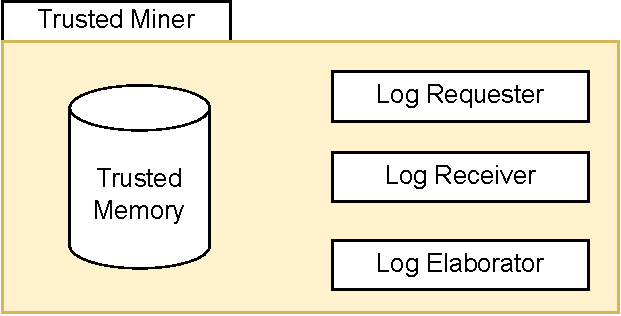
\includegraphics[width=7cm]{content/figures/Trusted_miner.pdf}
\caption{Modules of the Trusted Miner component running inside Trusted Execution Environments}
\label{fig:implementation}
\end{figure}
\subsubsection{Trusted Miner}
In our solution, \texttt{Trusted Execution Environments} are the key technologies that shelter external event logs inside an \texttt{Organization}'s system by preserving data confidentiality and integrity. The \texttt{Trusted Miner} component is a trusted application running inside the \texttt{Trusted Execution Environment} that makes its source code and data tamper-proof. The main goal of this component is to allow miner \texttt{Organization}s to execute process mining algorithms using %local event logs alongside 
event logs retrieved from provider \texttt{Organization}s, offering fair data utilization to the latters. In \cref{fig:trusted_miner}, we show an high level schematization of \texttt{Trusted Miner}s in which we distinguish four different modules: the \texttt{Trusted Memory}, the \texttt{Log Requester}, the \texttt{Log Receiver}, and the \texttt{Log Elaborator}.

Data contained in event logs belonging to provider \texttt{Organizaition}s are stored by miners in the \texttt{Trusted Memory}. This module relies on an hardware-encrypted zone of the cpu which makes event log manipuluations impossible from outside the \texttt{Trusted Execution Environment}. Modules of the \texttt{Trusted Miner} are the only entities enabled to access data stored in the \texttt{Trusted Memory}. Referring to our motivating scenario, the only way for the hospital to use the event logs retrieved from the specialized clinic is via the secure procedures offered by its \texttt{Trusted Miner}.

As we will see in \cref{sec:architecture:workflow}, the \texttt{Log Requester} and the \texttt{Log Receiver} are the fundamental modules that we employee during the event log exchange. \texttt{Log Requester}s initalize the exchange procedure and sends authenticable data requests to the \texttt{Data Provision} module of log providers. The \texttt{Log Receiver} collects event logs sent by \texttt{Log Providers} and store them in the \texttt{Trusted Memory}. This module offers methodologies that allow \texttt{Log Providers} to perform the remote attestation and verify the trustworthiness of the miner. According to our running example, the hospital's \texttt{Log Receiver} must prove its trusted nature to the clinc and the pharmaceutical company's \texttt{Log Provider} before receiving event logs, showing that it is actually running in a \texttt{Trusted Execution Environment}.

The \texttt{Log Elaborator} is the core module of the \texttt{Trusted Miner}. It collects the logic to run process mining algorithms in the \texttt{Trusted Execution Environment}. It support the integration of different family of tecniques such as \textit{process discovery}~\cite{citation}, \textit{conformance checking}~\cite{citation} and \textit{performance analysis}~\cite{ciation}. When activated, the \texttt{Log Elaborator} interacts with the \texttt{Trusted Memory} in order to access external event logs stored inside the \texttt{Trusted Execution Environment}. These are integrated with the local event log by the \texttt{Log Elaborator} via the merging procedure. During the merging, the \texttt{Log Elaborator} enriches local traces with events belonging to logs retrieved from partner \texttt{Organization}s. The integrity of the process mining tecniques that we implemented in the \texttt{Log Elaborator} is guaranteed by the \texttt{Trusted Execution Environment} that prevents malicious code manipulations from the running operative system.
Mentioning our motivating scenario, the \texttt{Log Elaborator} inside the \texttt{Trusted Miner} of the hospital merges the traces 




































\subsection{Workflow}
\label{sec:architecture:workflow}
\subsubsection{Initialization}
\subsubsection{Data Exchange}
\subsubsection{Data Elaboration}



